%\documentclass[handout]{ximera}
\documentclass[nooutcomes]{ximera}

\usepackage{gensymb}
\usepackage{tabularx}
\usepackage{mdframed}
\usepackage{pdfpages}
%\usepackage{chngcntr}

\let\problem\relax
\let\endproblem\relax

\newcommand{\property}[2]{#1#2}




\newtheoremstyle{SlantTheorem}{\topsep}{\fill}%%% space between body and thm
 {\slshape}                      %%% Thm body font
 {}                              %%% Indent amount (empty = no indent)
 {\bfseries\sffamily}            %%% Thm head font
 {}                              %%% Punctuation after thm head
 {3ex}                           %%% Space after thm head
 {\thmname{#1}\thmnumber{ #2}\thmnote{ \bfseries(#3)}} %%% Thm head spec
\theoremstyle{SlantTheorem}
\newtheorem{problem}{Problem}[]

%\counterwithin*{problem}{section}



%%%%%%%%%%%%%%%%%%%%%%%%%%%%Jenny's code%%%%%%%%%%%%%%%%%%%%

%%% Solution environment
%\newenvironment{solution}{
%\ifhandout\setbox0\vbox\bgroup\else
%\begin{trivlist}\item[\hskip \labelsep\small\itshape\bfseries Solution\hspace{2ex}]
%\par\noindent\upshape\small
%\fi}
%{\ifhandout\egroup\else
%\end{trivlist}
%\fi}
%
%
%%% instructorIntro environment
%\ifhandout
%\newenvironment{instructorIntro}[1][false]%
%{%
%\def\givenatend{\boolean{#1}}\ifthenelse{\boolean{#1}}{\begin{trivlist}\item}{\setbox0\vbox\bgroup}{}
%}
%{%
%\ifthenelse{\givenatend}{\end{trivlist}}{\egroup}{}
%}
%\else
%\newenvironment{instructorIntro}[1][false]%
%{%
%  \ifthenelse{\boolean{#1}}{\begin{trivlist}\item[\hskip \labelsep\bfseries Instructor Notes:\hspace{2ex}]}
%{\begin{trivlist}\item[\hskip \labelsep\bfseries Instructor Notes:\hspace{2ex}]}
%{}
%}
%% %% line at the bottom} 
%{\end{trivlist}\par\addvspace{.5ex}\nobreak\noindent\hung} 
%\fi
%
%


\let\instructorNotes\relax
\let\endinstructorNotes\relax
%%% instructorNotes environment
\ifhandout
\newenvironment{instructorNotes}[1][false]%
{%
\def\givenatend{\boolean{#1}}\ifthenelse{\boolean{#1}}{\begin{trivlist}\item}{\setbox0\vbox\bgroup}{}
}
{%
\ifthenelse{\givenatend}{\end{trivlist}}{\egroup}{}
}
\else
\newenvironment{instructorNotes}[1][false]%
{%
  \ifthenelse{\boolean{#1}}{\begin{trivlist}\item[\hskip \labelsep\bfseries {\Large Instructor Notes: \\} \hspace{\textwidth} ]}
{\begin{trivlist}\item[\hskip \labelsep\bfseries {\Large Instructor Notes: \\} \hspace{\textwidth} ]}
{}
}
{\end{trivlist}}
\fi


%% Suggested Timing
\newcommand{\timing}[1]{{\bf Suggested Timing: \hspace{2ex}} #1}




\hypersetup{
    colorlinks=true,       % false: boxed links; true: colored links
    linkcolor=blue,          % color of internal links (change box color with linkbordercolor)
    citecolor=green,        % color of links to bibliography
    filecolor=magenta,      % color of file links
    urlcolor=cyan           % color of external links
}

\title{Rep-Tiles Repeated}
\author{Bart Snapp and Brad Findell}

\outcome{Learning outcome goes here.}

\begin{document}
\begin{abstract}
  We further our study of rep-tiles.
\end{abstract}
\maketitle


\begin{teachingnote}
Materials:  Scissors and printed versions of the figures so that students can cut out already drawn ones.   
\end{teachingnote}

\begin{problem}
With a separate sheet of graph paper, draw and cut out the following polygons:
\begin{image}
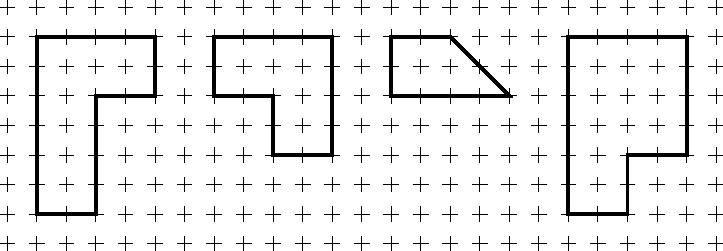
\includegraphics{rep-4-tile1.pdf}
\end{image}
Working with a partner, show that each of these polygons is a rep-4-tile.
\end{problem}

\begin{problem}
For each rep-tile above, compute the perimeter and area. In each case,
how does this relate to the perimeter and area of the larger polygon?
\end{problem}


\begin{problem}
With a separate sheet of paper, trace and cut out the following
polygons:
\begin{image}
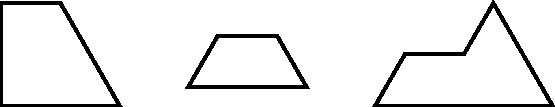
\includegraphics{rep-4-tile2.pdf}
\end{image}
Working with a partner, show that each of these polygons is a rep-4-tile.
\end{problem}


\begin{problem}
Explain why every rectangle whose sides have ratio $1:\sqrt{n}$ is a
rep-$n$-tile.
\end{problem}

\begin{problem}
Explain how you know that any polygonal rep-tile will tessellate the plane.
\end{problem}

\begin{problem}
Give an example of a polygon that tessellates the plane that is not a
rep-tile.
\end{problem}


\begin{problem}
Every tessellation made by rep-tiles will have \index{symmetry of
scale}\textbf{symmetry of scale}. What does it mean to have \textit{symmetry of scale}?
\end{problem}

\begin{problem}
Consider the tessellations made by rep-tiles you've seen so far. What
other symmetries do they have?
\end{problem}

\begin{problem}
Do you think you can have a tessellation that has symmetry of scale
but no other symmetries?
\end{problem}

\end{document}
